% !TeX spellcheck = en_GB
\ifcsname SlidesDistr\endcsname%
	\documentclass[handout,aspectratio=169]{beamer}
\else%
	\documentclass[aspectratio=169]{beamer}
\fi%
\input{../syde556_lecture_slides_preamble}

\date{Sept 18 \& 23, 2024}
\title{SYDE 556/750 \\ Simulating Neurobiological Systems \\ Lecture 4: Temporal Representations}

\begin{document}

\begin{frame}{}
	\vspace{0.5cm}
	\begin{columns}[c]
		\column{0.6\textwidth}
		\MakeTitle
		\column{0.4\textwidth}
		\includegraphics[width=\textwidth]{media/camille_gravis_captive_balloon_with_clock_face_small.jpg}
	\end{columns}
\end{frame}

\begin{frame}{Reminder: The LIF Neuron}
	\begin{columns}[c]
		\column{0.6\textwidth}
		\includegraphics[width=\textwidth]{media/lif_neuron_ramp.pdf}
		\column{0.4\textwidth}
		\includegraphics[width=\textwidth]{media/lif_circuit.pdf}
	\end{columns}
	\begin{align*}
		\frac{\mathrm{d}}{\mathrm{d}t} v(t) &= -\frac{1}{\tau_\mathrm{RC}} \big( v(t) - J \big) \,, \quad &\text{if } v(t) &< 1\,, \\
		v(t) &\gets \delta(t - t_\mathrm{th}) \,, &\text{if } t &= t_\mathrm{th} \,,\\
		v(t) &\gets 0 \,, &\text{if } t &> t_\mathrm{th} \text{ and } t \geq t_\mathrm{th} + \tau_\mathrm{ref} \,,
	\end{align*}
\end{frame}

\begin{frame}{Temporal Decoding}
	\begin{itemize}
		\setlength{\itemsep}{0.25cm}
		\item For population decoders, we needed to integrate their responses, $\mathbf{a}(\mathbf{x})$,  over the represented variable, $\mathbf{x}$.
		\item <2->For temporal decoders, we will likely want to integrate their responses, $\mathbf{a}(t)$,  over the represented variable, $\mathbf{x}(t)$.
		\item <3->What space do we want to sample to estimate the integrals?
    \end{itemize}
\end{frame}

\begin{frame}{Random Signals}
	\begin{overlayarea}{\textwidth}{0.9\textheight}
		\begin{columns}
			\column{0.75\textwidth}
			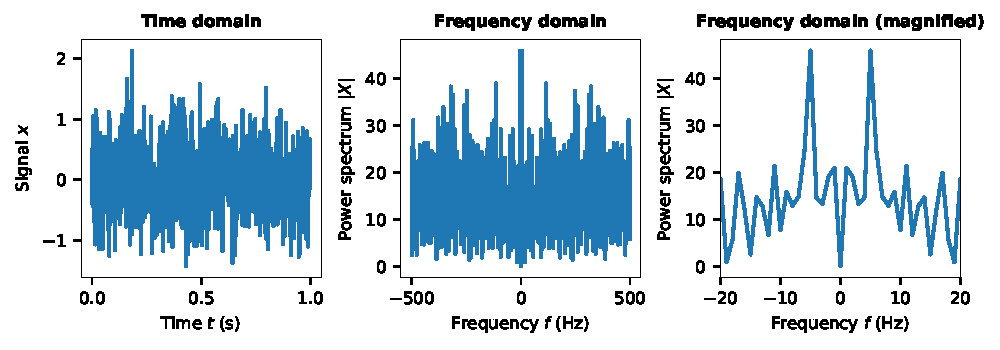
\includegraphics[width=\textwidth]{media/white_noise.pdf}
			\column{0.25\textwidth}
			\hl{White Noise}\\
			(zero mean)
		\end{columns}
		\only<2>{\begin{columns}
			\column{0.75\textwidth}
			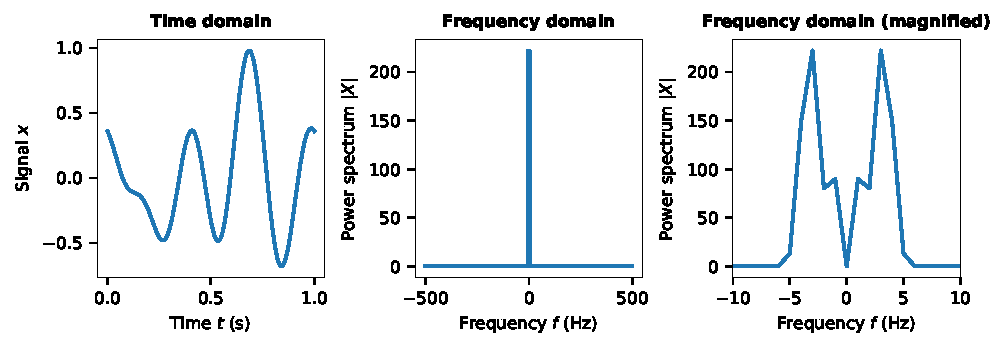
\includegraphics[width=\textwidth]{media/white_noise_5hz.pdf}
			\column{0.25\textwidth}
			\hl{Bandlimited}\\White Noise\\
			(zero mean,\\\SI{5}{\hertz} bandwidth)
		\end{columns}}
		\only<3>{\begin{columns}
			\column{0.75\textwidth}
			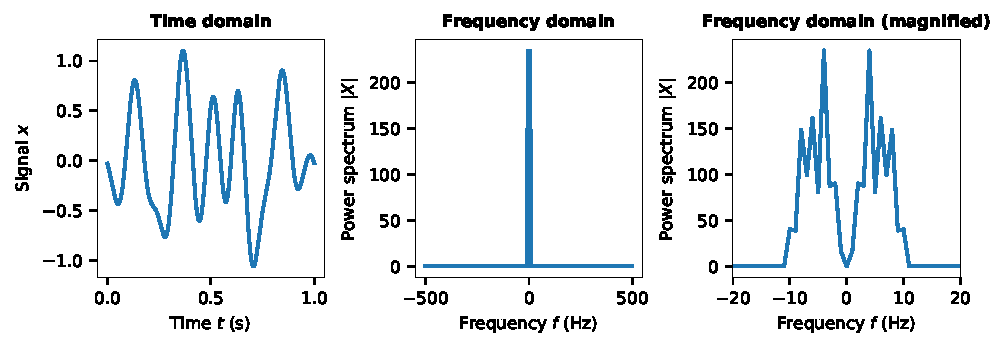
\includegraphics[width=\textwidth]{media/white_noise_10hz.pdf}
			\column{0.25\textwidth}
			\hl{Bandlimited}\\White Noise\\
			(zero mean,\\\SI{10}{\hertz} bandwidth)
			\end{columns}}
	\end{overlayarea}
\end{frame}

\begin{frame}{Temporal Decoding of Two Neurons - Weighted Spikes}
	\includegraphics[width=0.4\textwidth]{media/two_neurons_tuning_curves.pdf}%
	\includegraphics[width=0.6\textwidth]{media/two_neurons_spike_train.pdf}
\end{frame}

\begin{frame}{Temporal Decoding of One Hundred Neurons - Weighted Spikes}
	\includegraphics[width=0.4\textwidth]{media/hundred_neurons_tuning_curves.pdf}%
	\includegraphics[width=0.6\textwidth]{media/hundred_neurons_spike_train.pdf}
\end{frame}

\begin{frame}{Filtering by Convolution}
	\begin{columns}
		\column{0.5\textwidth}
		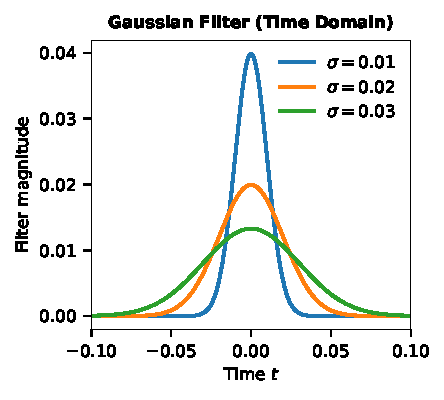
\includegraphics[width=\textwidth]{media/gaussian_filters.pdf}
		\column{0.5\textwidth}
		\begin{block}{Gaussian Filter}
			\begin{align*}
				h(t) &= c \exp \left( \frac{-t^2}{\sigma^2} \right) \\
				\text{where }  &~c \text{ chosen s.t. } {\textstyle \int_{-\infty}^\infty h(t) \,\mathrm{d}t = 1}
			\end{align*}
		\end{block}
		\begin{block}{Convolution}
			\begin{align*}
				\big( f \ast h \big)(t) &= \int_{-\infty}^{\infty} f(t - t') h(t') \,\mathrm{d}t'
			\end{align*}
		\end{block}
	\end{columns}
\end{frame}

\begin{frame}{Filtering a Spike Train}
	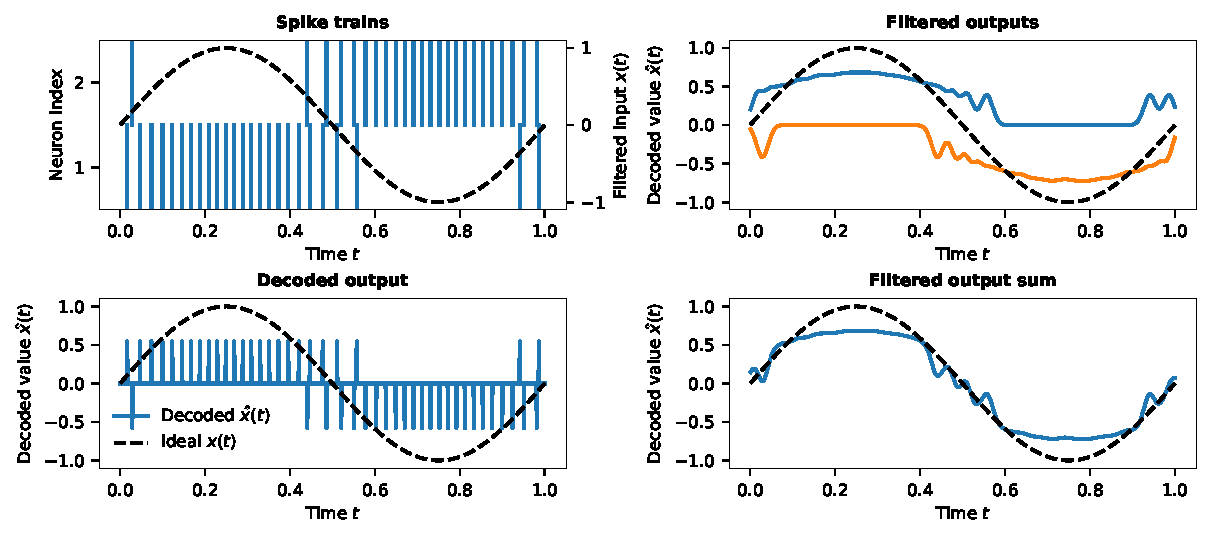
\includegraphics[width=\textwidth]{media/two_neurons_filtered.pdf}
\end{frame}

\begin{frame}{Filtering a Spike Train for a Random Signal}
	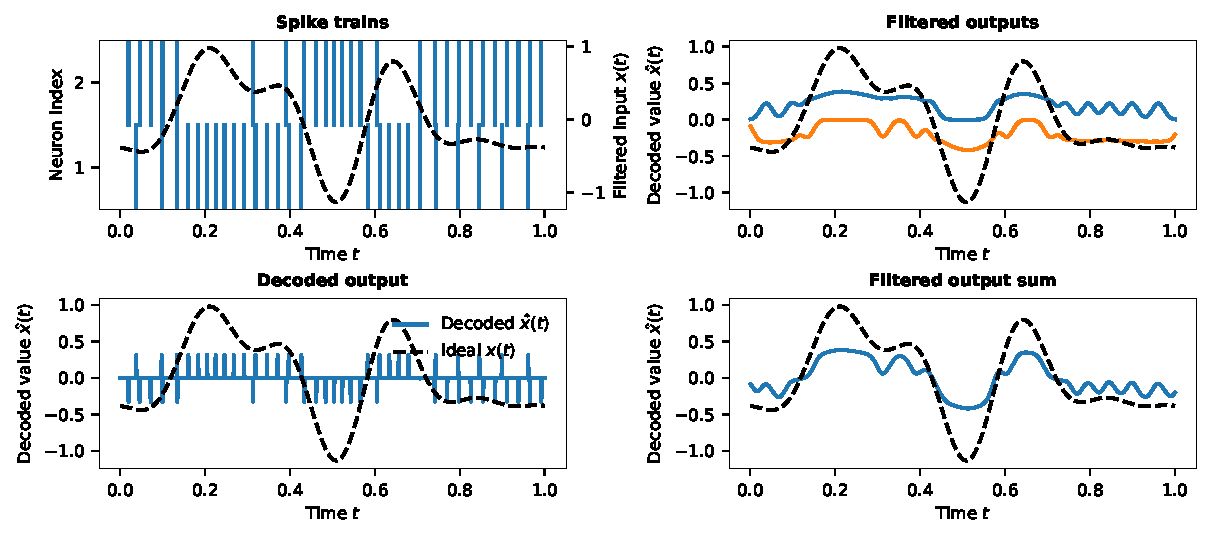
\includegraphics[width=\textwidth]{media/two_neurons_filtered_white_noise.pdf}
\end{frame}

\begin{frame}{Optimal Filter}
	\centering
	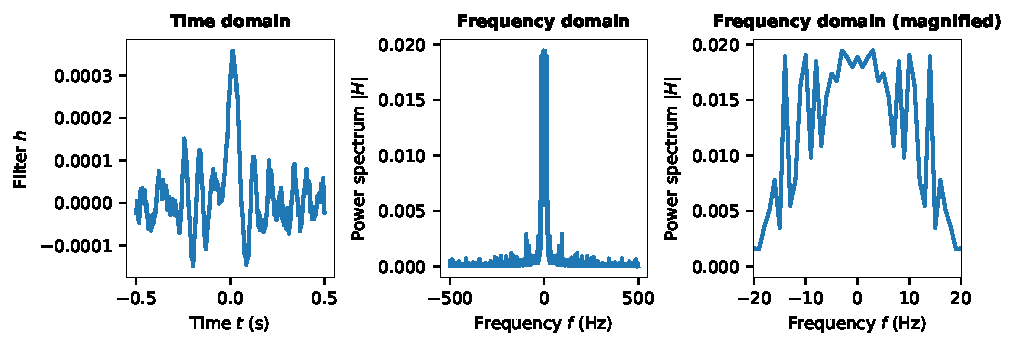
\includegraphics[width=\textwidth]{media/optimal_filter.pdf}\\
	$$H(\omega) = {{X(\omega) \overline{R}(\omega)} \over {|R(\omega)|^2}}$$
\end{frame}

\begin{frame}{Filtering a Spike Train for a Random Signal (Optimal Filter)}
	\includegraphics<1>[width=\textwidth]{media/two_neurons_filtered_white_noise.pdf}
	\includegraphics<2>[width=\textwidth]{media/two_neurons_filtered_optimal_simple.pdf}
	\includegraphics<3>[width=\textwidth]{media/two_neurons_filtered_optimal_simple_2.pdf}
	\includegraphics<4>[width=\textwidth]{media/two_neurons_filtered_optimal_simple_3.pdf}
\end{frame}

\begin{frame}{Optimal Filter (Improved)}
	\centering
	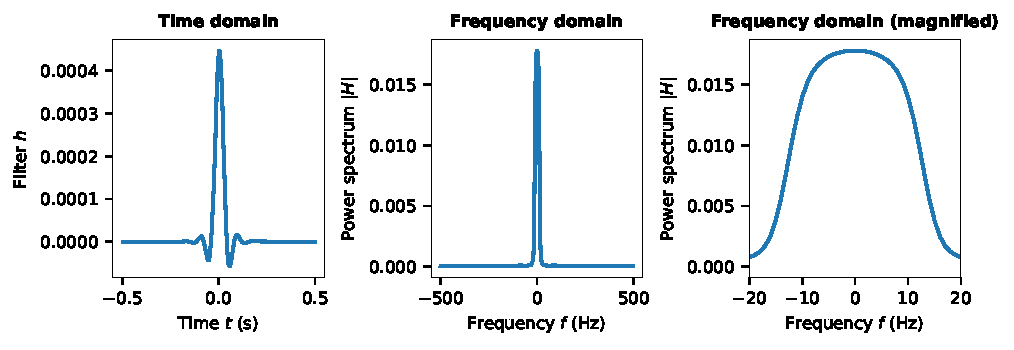
\includegraphics[width=\textwidth]{media/optimal_filter_improved.pdf}\\
	$$H(\omega) = {{X(\omega) \overline{R}(\omega)} \ast W(\omega) \over {|R(\omega)|^2} \ast W(\omega)} $$
\end{frame}

\begin{frame}{Filtering a Spike Train for a Random Signal (Improved Optimal Filter)}
	\includegraphics<1>[width=\textwidth]{media/two_neurons_filtered_optimal_simple.pdf}
	\includegraphics<2>[width=\textwidth]{media/two_neurons_filtered_optimal.pdf}
	\includegraphics<3>[width=\textwidth]{media/two_neurons_filtered_optimal_2.pdf}
	\includegraphics<4>[width=\textwidth]{media/two_neurons_filtered_optimal_3.pdf}
\end{frame}

\begin{frame}{Pros and Cons of the Optimal Filter}
	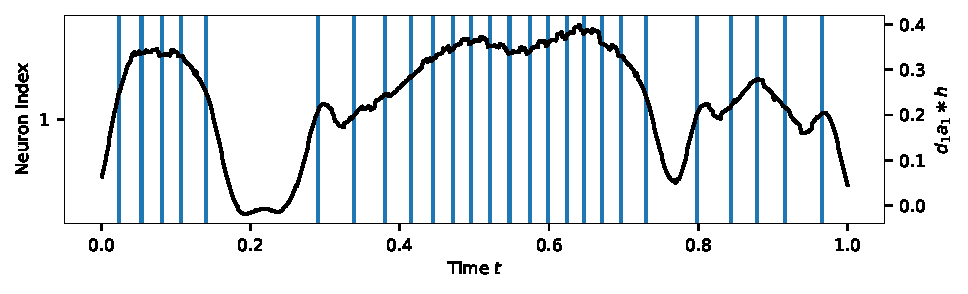
\includegraphics[width=\textwidth]{media/filter_magnification.pdf}
	\begin{columns}[t]
		\column{0.5\textwidth}
		\begin{itemize}
			\item<2->[\OPlus] \textbf{Precise}\\Good for analysing data after the fact
		\end{itemize}
		\column{0.5\textwidth}
		\begin{itemize}
			\item<3->[\OMinus] \hl{Non-causal}\\Does not describe a biological process
		\end{itemize}
	\end{columns}
	\vspace{0.5cm}
	\begin{overlayarea}{\textwidth}{0.5cm}
		\centering
		\quotefont\large
		\only<4->{We need to find a mechanism that low-pass filters spikes over time!}
	\end{overlayarea}
\end{frame}

\begin{frame}{Synapses as Filters}
	\centering
	\includegraphics[width=0.375\textwidth]{media/synapse_schematic.pdf}~~%
	\includegraphics[width=0.55\textwidth]{media/burke_1967_epsp.png}\\[0.5cm]
	\centering
	\begin{overlayarea}{\textwidth}{0.5cm}
		\centering
		\only<2->{\quotefont\large
		\hl{Post-synaptic currents (EPSCs, IPSCs) are low-pass filtered spike trains!}}
	\end{overlayarea}
\end{frame}

\begin{frame}{Exponential Low-Pass Filter (I)}
	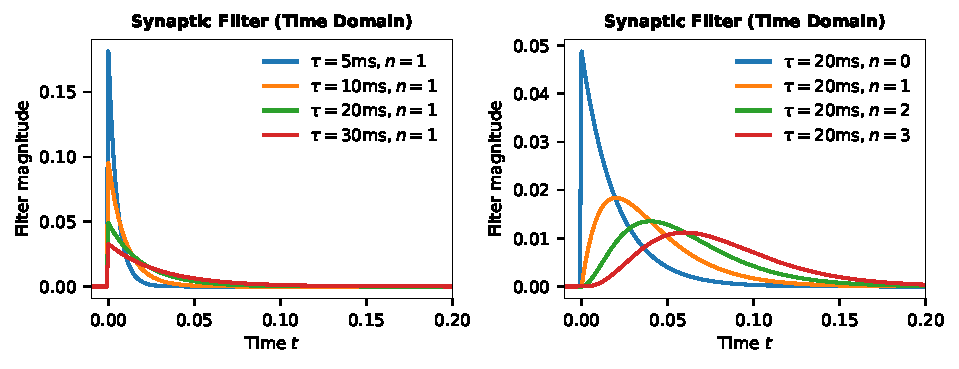
\includegraphics[width=\textwidth]{media/synaptic_filters.pdf}
	\begin{align*}
			h(t) &= \begin{cases}
		c^{-1} t^n \exp^{-t / \tau} & \text{if } t \geq 0 \,,\\
		0 & \text{otherwise}\,,
		\end{cases}
		&& \text{where } c = \int_{0}^\infty t^n \exp^{-t / \tau} \,\mathrm{d}t \,.
	\end{align*}
\end{frame}

\begin{frame}{Exponential Low-Pass Filter (II)}
	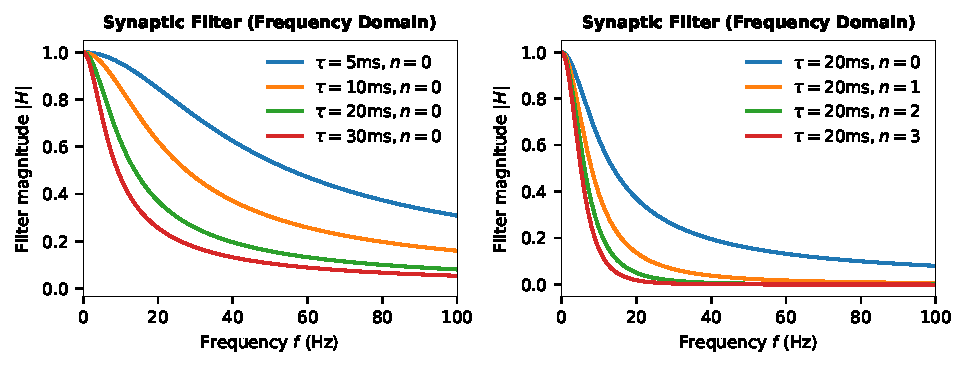
\includegraphics[width=\textwidth]{media/synaptic_filters_freq.pdf}
	\begin{align*}
	h(t) &= \begin{cases}
	c^{-1} t^n \exp^{-t / \tau} & \text{if } t \geq 0 \,,\\
	0 & \text{otherwise}\,,
	\end{cases}
	&& \text{where } c = \int_{0}^\infty t^n \exp^{-t / \tau} \,\mathrm{d}t \,.
	\end{align*}
\end{frame}

\begin{frame}{Example: Synaptic Filter for Two Neurons}
	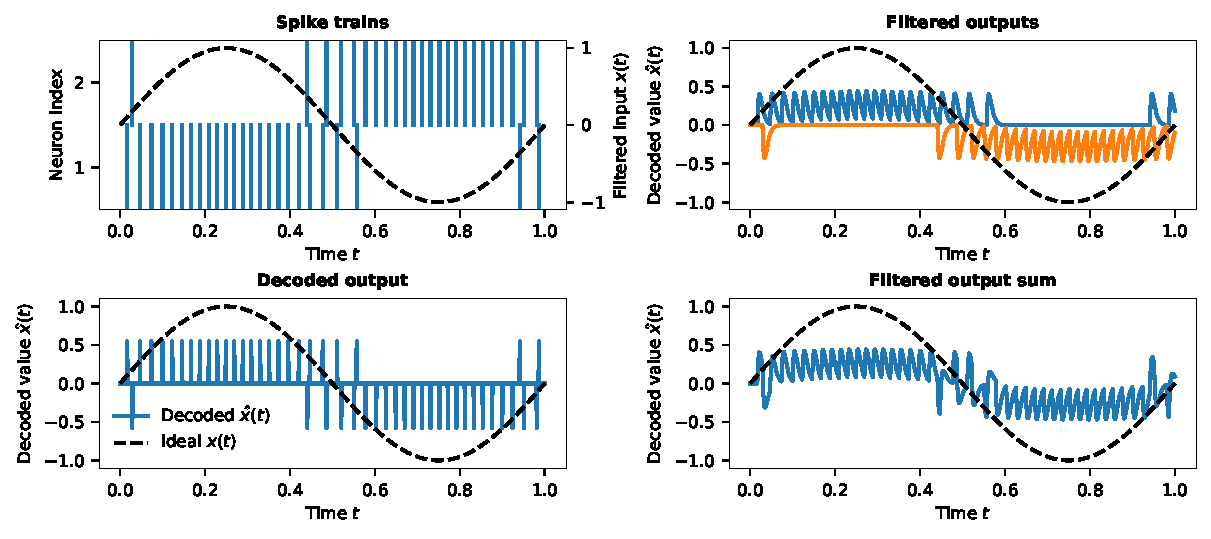
\includegraphics[width=\textwidth]{media/two_neurons_synaptic_filter.pdf}\\
	\centering $\tau = \SI{5}{\milli\second}, n = 1$
\end{frame}

\begin{frame}{Example: Synaptic Filter for One Hundred Neurons}
	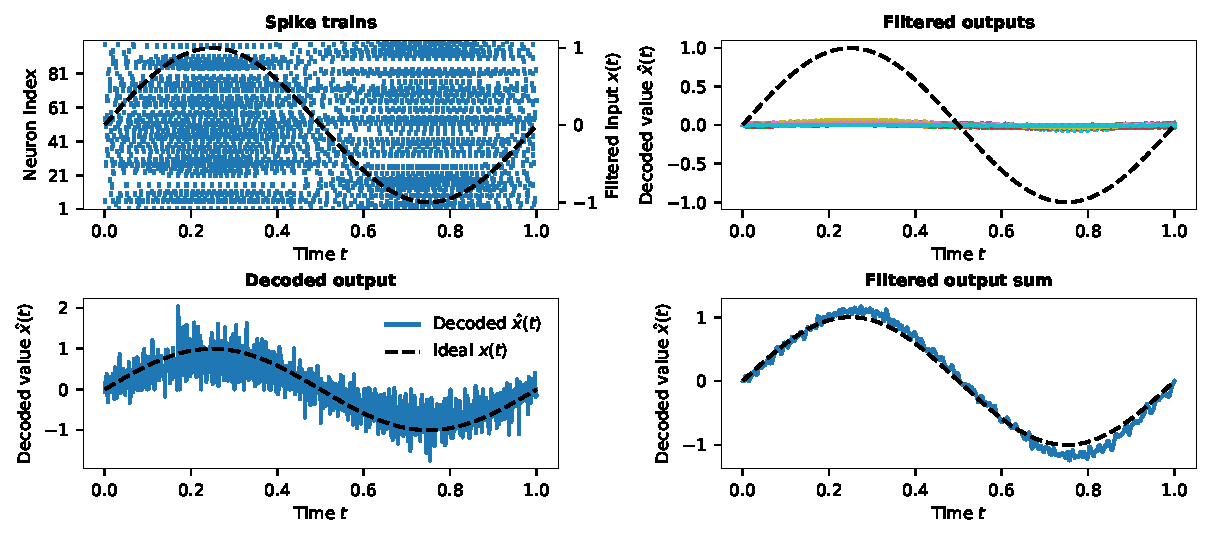
\includegraphics[width=\textwidth]{media/n_neurons_synaptic_filter.pdf}
	\centering $\tau = \SI{5}{\milli\second}, n = 1$
\end{frame}

\backupbegin

\begin{frame}[noframenumbering]{Image sources}
	\small
	\textbf{Title slide}\\\enquote{Captive balloon with clock face and bell, floating above the Eiffel Tower, Paris, France.}\\Author: Camille Grávis, between 1889 and 1900.\\From \href{https://commons.wikimedia.org/wiki/File:Camille_Gr\%C3\%A1vis,_Captive_balloon_with_clock_face_and_bell,_floating_above_the_Eiffel_Tower,_Paris,_France.jpg}{Wikimedia}.
\end{frame}


\backupend

\end{document}
